\documentclass[a4paper, 12pt]{article}
\usepackage[utf8]{inputenc}
\usepackage{graphicx}
\usepackage{amsmath}
\usepackage{amssymb}
\usepackage{geometry}
\usepackage{hyperref}
\geometry{margin=1in}

\title{Workflow Proposal for Moodle Formula Question Generation Application}
\author{Otito Mbelu}
\date{\today}

\begin{document}

\maketitle

\begin{abstract}
This proposal outlines the objectives, methodology, and timeline for the design and deployment of the afore-mentioned Application. 
The goal of this project is to create a user friendly application that can generate a valid Moodle formula question from a given set of 
parameters. These parameters may come in the form of the NFQ level of the question targets or other customizable parameters.  
\end{abstract}

\tableofcontents
\newpage

\section{Introduction}
Given the already noted complexities involved in setting up a Moodle question bank, it is important to have a tool that can automate the process
given a set of parameters. Also given limited time and resources available to carry out the project, effort will be directed towards the generation 
of XML files that can be imported into Moodle and thus avoid the need to create a plugin that integrates directly into Moodle given limited documentation
and documented anomalies on the Moodle Plugin API. 

\section{Background}
After a careful review of three different question samples, the following observations were made. 
\begin{itemize}
    \item The questions have a specific structure. 
    \item The questions are in a specific format.
    \item The only structural difference between questions were observed on the number of sub questions contained. In this case,
        a variable number of `answers' tags were present.
\end{itemize}
As such the following steps will be taken to generate the questions given two different scenarios.
\begin{figure}[h]
    \begin{center}
       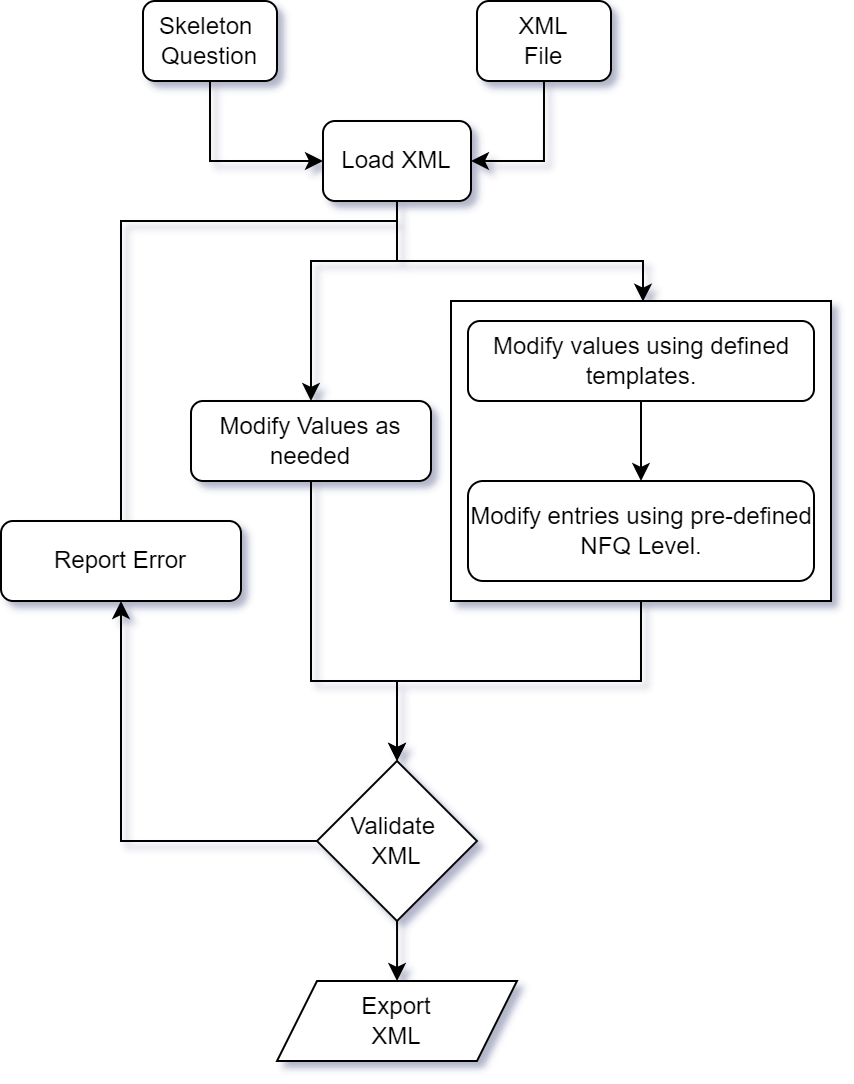
\includegraphics[width=8cm]{images/app_diag.png} 
       \caption[]{Application Flow Diagram}\label{fig:app_diag}
    \end{center}
\end{figure}


\subsection{Scenario 1} Generating a question from scratch
\begin{itemize}
    \item \textbf{Step 1:} Create a wizard-like interface that will allow the user to input relevant parameters of the questions. 
    \item \textbf{Step 2:} Generate the XML file based on the parameters input by the user.
\end{itemize} 
\subsection{Scenario 2} Generating a question from a template
\begin{itemize}    
    \item \textbf{Step 1:} Select a template from a list of templates. 
    \item \textbf{Step 2:} Modify the template based on the parameters input by the user. Making cascading group of changes will also be possible
    using dropdowns.
\end{itemize}

\section{Objectives}
The overall objective of this project will be to enable educators create Moodle questions on the fly. Automating this process will involve understudying
the structure of the XML files that represent the Moodle questions and creating a user-friendly interface that can generate these files given minimal input.
The following objectives will be pursued from the design point of view to achieve these functionalities.

\begin{itemize}
    \item Create a validation system that will ensure that the XML files generated are valid. This will involve matching all the declared variables with 
    the correctness criteria of the Moodle XML schema and also the declared placeholders with the correct matching text.
    \item Dynamically generate several sub-questions on the go, using relevant input controls like `buttons', `fields', `checkboxes', etc. 
    \item Create grading variables and correctness logic using a user-friendly interface.
\end{itemize}

\section{Technology Review}
\subsection{Java Desktop Application} 
A Java desktop application was developed as a prototype to showcase possible solution to the problem. However, deploying such application requires 
distributing binary files for installation and running on user's local machine. And the source code cannot be reused to for front-end web application 
solution as there is no viable Java front-end web framework. 

\subsection{Web Application - Angular Web Framework}

A web application offers the advantage of being deployable and accessible over the internet. This will allow easy access to the application to any user without
the need to run any installation on their local machine as the application is accessible through any browser running on any platform, mobile devices inclusive. 


\subsection{Microsoft PowerApp}

Microsoft PowerApp also offers another accessible solution with the added advantage of being integrated into Microsoft Teams Application. However, the program 
logic involved in implementing all the required functionalities seems prohibitive on a PowerApp Canvas Application. 
These functionalities could however, be implemented using a backend service that does all the processing while the PowerApp is utilized solely as a 
presentation interface. 


\section{Methodology}

The project is projected to go through 3 stages that involves creating a skeletal interface that shows all the properties of a given question, 
implementing automation functionalities that generates sub-questions, formula, correctness logic, etc. and finally testing and deployment of the 
application. 
Depending on the availability of time and the need to develop a PowerApp application, a backend implementation of the application functionalities may be 
implemented to allow the development of a simple PowerApp interface that can be integrated with Microsoft Teams.

\begin{figure}[h]
    \begin{center}
       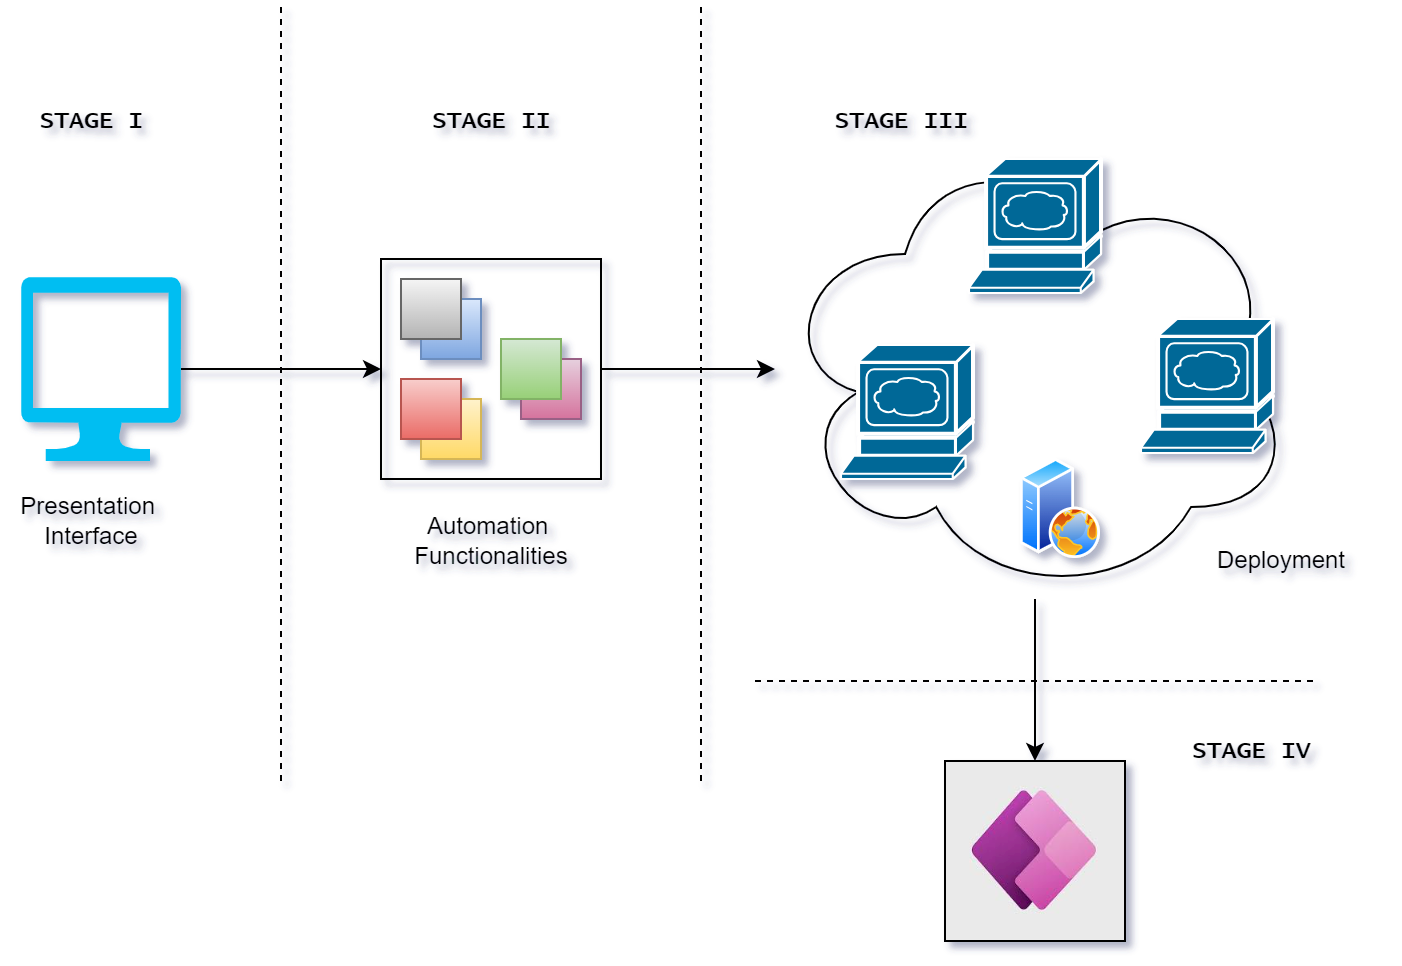
\includegraphics[width=12cm]{images/app_meth.png} 
       \caption[]{Application Design Stages}\label{fig:app_meth}
    \end{center}
\end{figure}
\section{Conclusion}
This document is only but a proposal and a probable course of action and is subject to change. More so, granular details of various stages mentioned
above will be analyzed and finalized as we make progress.

\end{document}
